\documentclass[a6paper, parskip=half, DIV=14, 12pt]{scrartcl}

\usepackage{aoa}

\usepackage{aoarules}


\begin{document}
{%
\thispagestyle{empty}
		\enlargethispage{3.5\baselineskip} % Move the bottom line (author and date) down a bit
\setmainfont[Scale=1.0]{Caslon Antique}
\begin{center}
\makeatletter
{\footnotesize Version \@version}
\makeatother


\vfill

{
\setmainfont[Scale=1.7]{Tradewinds}
\Huge
\textcolor{bandana}{Articles\hfill of\\Agreement}
}

\vspace{-0.5cm}

\tikz{\node[inner sep=0pt] {\includegraphics[height=8cm]{Images/pirate-ship-small.png}};}

\vfill{}

{
\setmainfont{Aquiline Two}
\Large
\textcolor{bandana}{Designed by Michael Purcell}
}
\end{center}
}

\newpage
\section*{Overview}
Articles of Agreement is a negotiation game for four to seven players that can be played in about thirty minutes.

You will play as the members of a pirate crew who are dividing some loot that you recently ... acquired.
In principle, you are all entitled to an equal share of that loot.
In practice, however, you can split the loot however you want \textendash{} provided that you can convince a majority of the crew to agree to the proposed allocation. 

%\begin{itemize}[leftmargin=*]
%\item Can you convince your crewmates to give you more than your fair share of the loot?
%\item Will you do the same for any of them in return?
%\item What will you do if your so-called friends decide to cheat you and keep all the loot for themselves?
%\end{itemize}

If you can secure the most valuable share of the loot, you will win the game and become one of history's most infamous pirates.

\bigskip

\bigskip

\begin{multicols}{2}
\section*{Components}
\begin{itemize}[leftmargin=*, nosep]
\item 70 cards
\begin{itemize}[leftmargin=*, nosep]
\item 62 treasure cards,
\item 7 character cards,
\item 1 captain card.
\end{itemize}
\end{itemize}
\vfill{}\null

\begin{center}
\includegraphics[width=0.4\textwidth]{Images/parrot-1.png}
\end{center}
\end{multicols}

\newpage

\section*{Set Up}
\begin{itemize}[leftmargin=*]
\item Separate the cards by type.
%\begin{itemize}[leftmargin=*, nosep]
%\item sixty-two loot cards (white),
%\item seven character cards (blue),
%\item one captain card (red).
%\end{itemize}
%\end{itemize}
%\begin{itemize}[leftmargin=*]
\item Shuffle the treasure cards.
\item Deal two treasure cards face down to each player.
%\item Shuffle the character cards.
%\item Deal one character card face up to each player.
\item Give the captain card face up to the player who most recently went sailing. %with the highest-numbered character card.
\end{itemize}

\bigskip

\bigskip

\begin{center}
%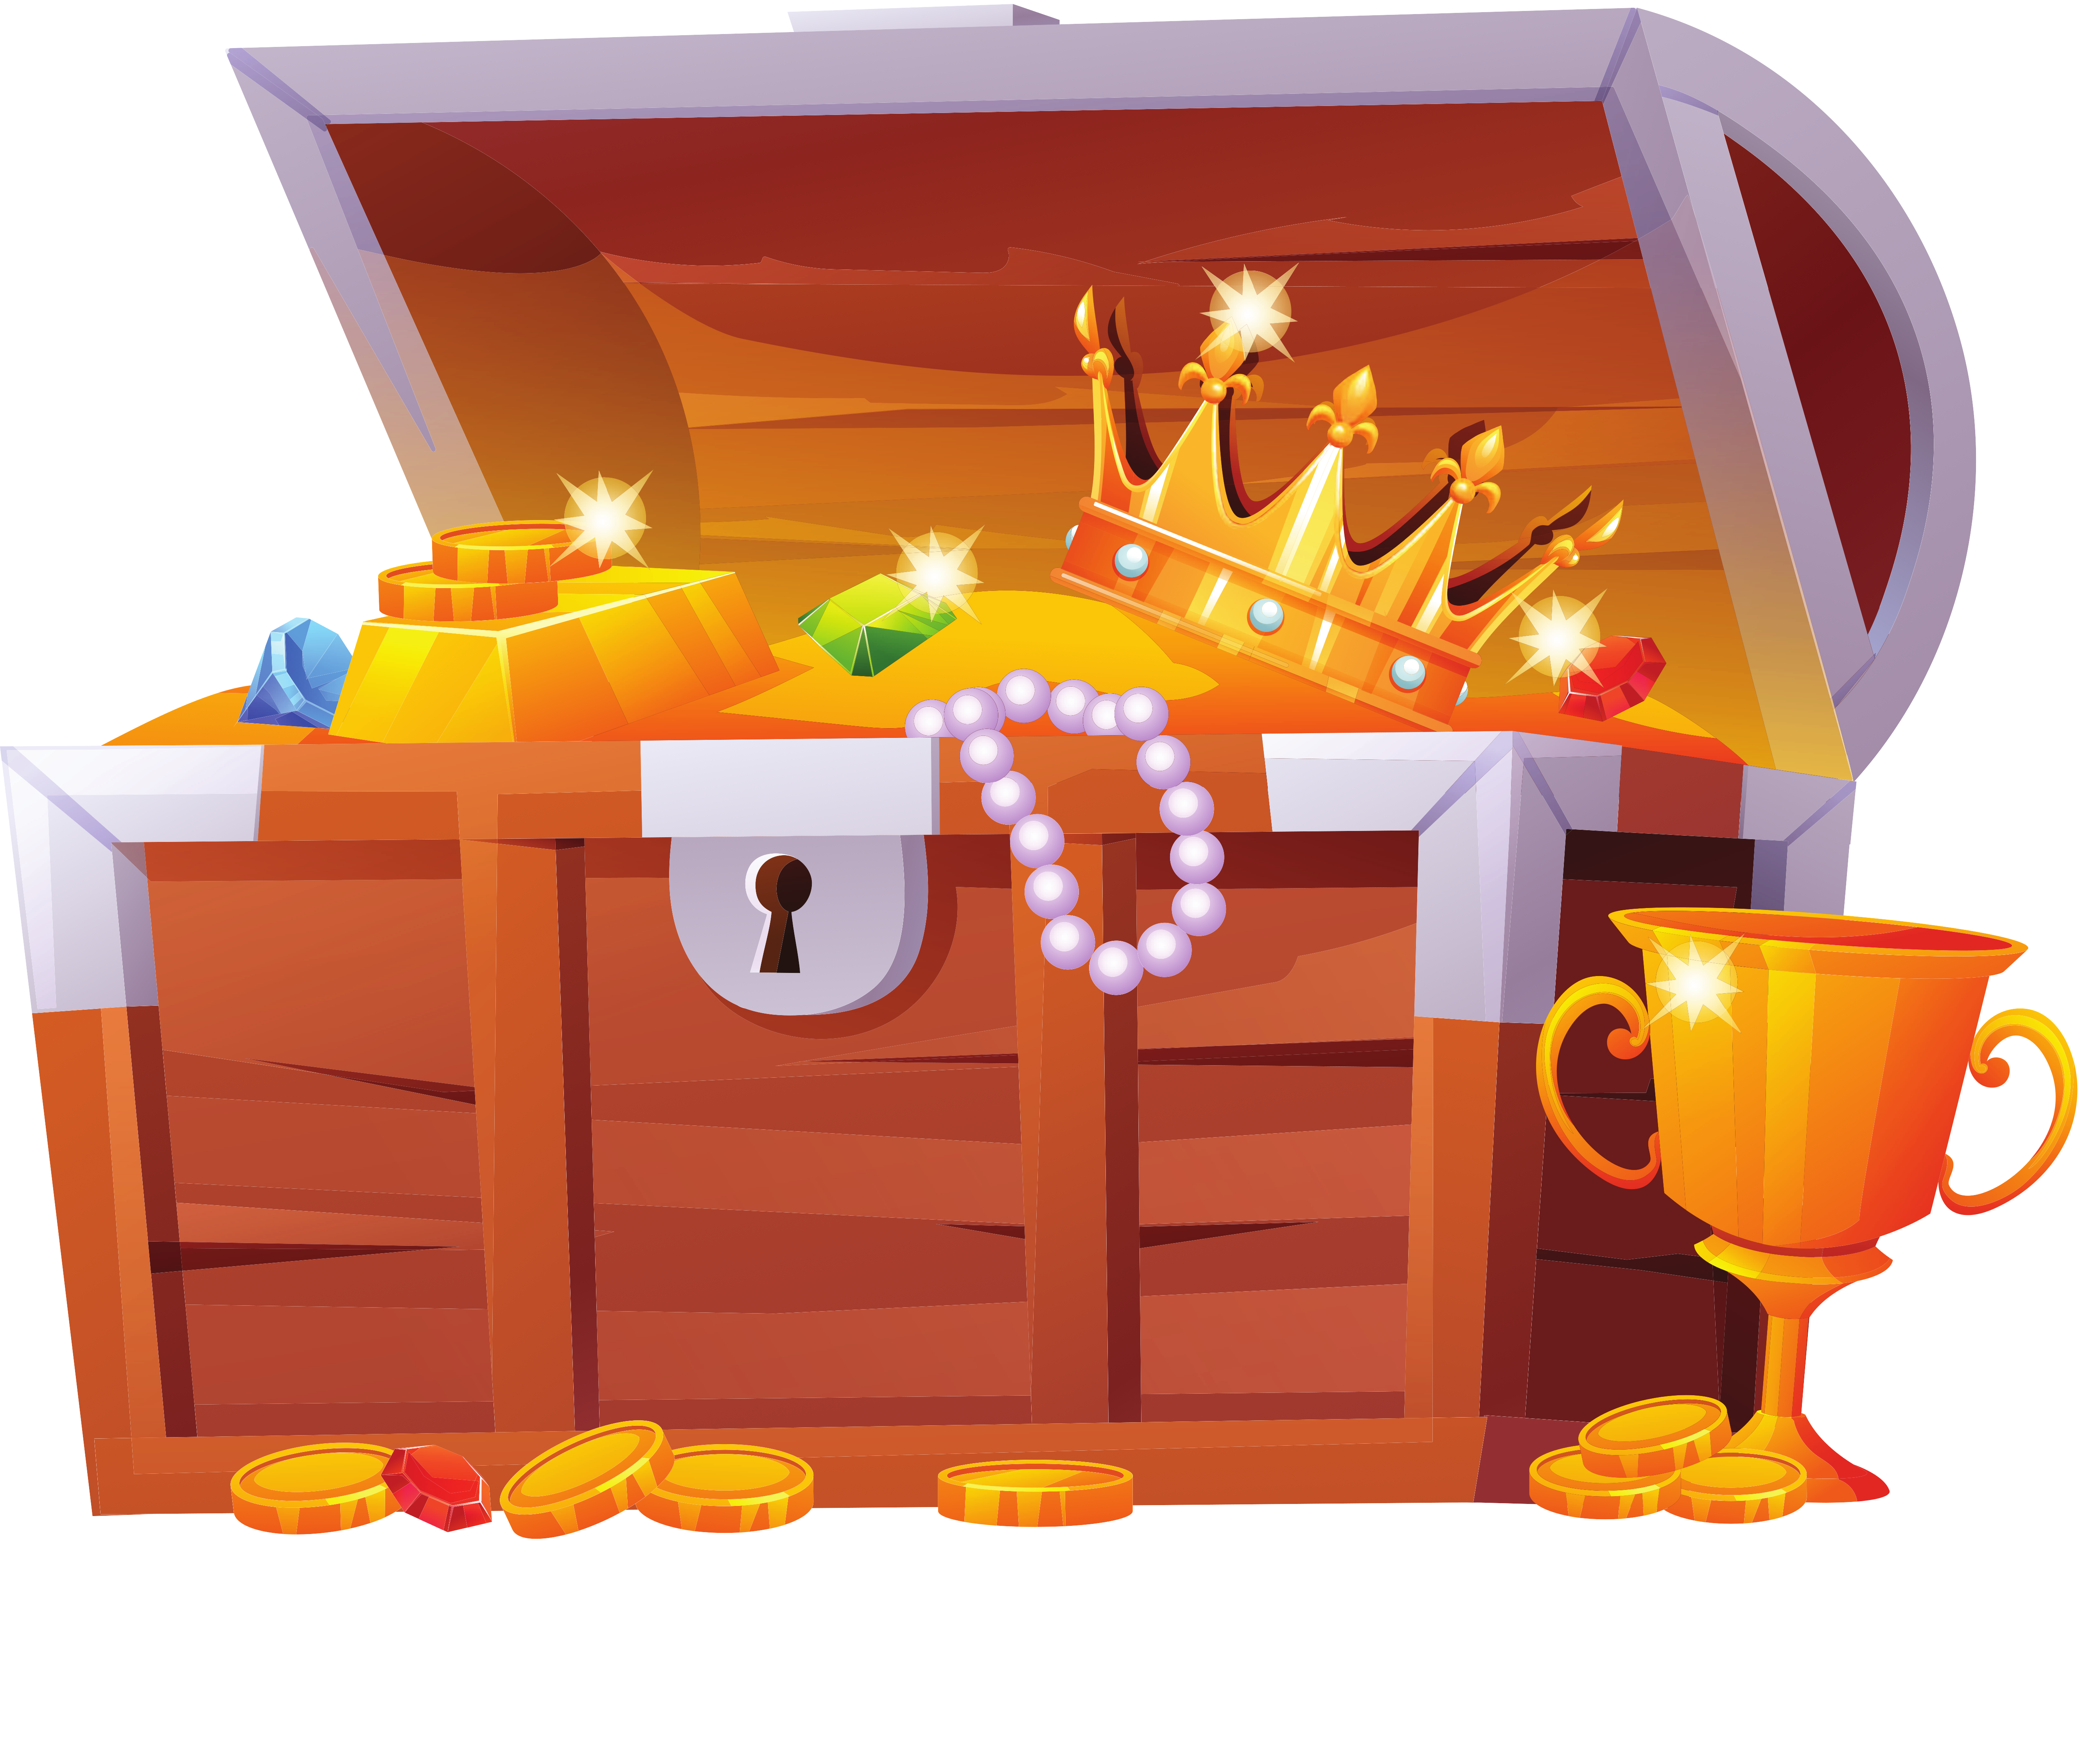
\includegraphics[width=0.7\textwidth]{Images/treasure-chest.png}


\includegraphics[height=4.75cm]{Images/pirate-7b.png}
\qquad
\includegraphics[height=4cm]{Images/pirate-1.png}
\qquad
\includegraphics[height=4.5cm]{Images/pirate-2.png}

\end{center}

\newpage

\section*{Characters}
Each character card is composed of a character number, a character portrait, and a character ability that can be used once per game.

Character abilities on lower-numbered character cards resolve earlier in the round than those on higher-numbered character cards.

The highest-numbered character will be the captain at the beginning of the game.

\vfill

\begin{center}

\includegraphics[height=4.75cm]{Images/pirate-7b.png}
\qquad
\includegraphics[height=4cm]{Images/pirate-1.png}
\qquad
\includegraphics[height=4.5cm]{Images/pirate-2.png}
\end{center}

\newpage

\section*{Gameplay}
The game is played over a series of six rounds, each of which consists of two or three phases: allocate, vote, and (depending on the outcome of the vote) mutiny.

\subsection*{Allocate}
The captain draws seven random treasure cards face up and proposes an allocation of those treasure cards.

The captain must assign a (possible empty) share of the treasure to each player including themself. Every treasure card must be included in exactly one share.

All players are encouraged to attempt to influence the captain while they try do decide on their proposed allocation.
Ultimately, however, the captain can propose any allocation they like. 

\begin{center}
\includegraphics[height=2cm]{Images/cannon.png} \quad \reflectbox{\includegraphics[height=2cm]{Images/cannon.png}}%\includegraphics[height=1.75cm]{Images/barrel.png} \includegraphics[height=1.75cm]{Images/barrel.png}
\end{center}

\newpage

\subsection*{Vote}
All players simultaneously vote on whether to accept the captain's proposed allocation or to reject it.

Each player must either vote \textit{Aye} to accept the captain's proposed allocation or \textit{Nay} to reject it.
Before the game, agree on how you will indicate your votes. A common choice is to use a ``thumbs up'' gesture to indicate \textit{Aye} and a ``thumbs down'' gesture to indicate \textit{Nay}.

\textbf{Note:} The captain must always vote to accept their own proposed allocation.

If a majority of the players voted \textit{Aye}:
\begin{itemize}[leftmargin=*]
\item Players who voted \textit{Aye} keep their allocated shares.
\item Players who voted \textit{Nay} get nothing. Nothing!\\They must discard their allocated shares.
\item The captain retains their position and will serve as captain again for the next round.
\end{itemize}

Otherwise, including the case of a tied vote, the players who voted \textit{Nay} mutiny.

\newpage

\subsection*{Mutiny}
During a mutiny, all players who voted \textit{Nay} during the voting phase this round become mutineers and seize control from the captain.
When they do, they must:
\begin{itemize}[leftmargin=*]
\item Propose an allocation for this round's treasure cards.
\item Choose a mutineer to become the new captain.
\end{itemize}

If the mutineers \textbf{unanimously} agree on both their proposed allocation and their nominee to become the new captain, the mutiny succeeds.
In that case:
\begin{itemize}[leftmargin=*]
\item All players keep their allocated shares.
\item The nominated mutineer becomes the new captain. Give the captain card to the new captain.
\end{itemize}

Otherwise, the mutiny does not succeed. In that case:
\begin{itemize}[leftmargin=*]
\item All of this round's treasures are discarded.
\item The previous captain retains their role.
\end{itemize}

\textbf{Note:} The mutineers can allocate shares to players who are not mutineers. If the mutiny succeeds, all players must keep the shares allocated to them by the mutineers.


\newpage

\section*{Scoring}
At the end of the final round, each player scores some number of points determined by the treasures they have collected throughout the game.

There are twelve types of treasure, each of which scores differently.
The scoring rules for each type of treasure are described on the {\setmainfont{Tradewinds}\scriptsize Scoring Summary} reference card and are displayed on the treasure cards themselves.

\section*{Game End}
After the sixth round ends, everyone has a final opportunity to use pistols and barrels.
Then, everyone should reveal all of their secret treasures.

Finally, each player should compute their final score.
The player with the highest score wins the game and will be remembered as one of history's most infamous pirates.






\vfill

\hrulefill

{\footnotesize \textbf{Design}: Michael Purcell \hfill \textbf{Contact}:~\href{mailto:mike@armiger.games}{mike@armiger.games}}

\begin{tabular}{ll}
\footnotesize{\doclicenseText} & \huge{\doclicenseIcon} \\
\end{tabular}

\newpage

\enlargethispage{2.0\baselineskip}
\section*{\phantom{a}\hfill{}Scoring Summary\hfill\phantom{a}}

\medskip

\begin{minipage}{1.5cm}
\tikz{\node[draw, thick, minimum width=1.5cm, minimum height=1.5cm, inner sep=0pt, rounded corners=3mm] at (0,0) {\includegraphics[width=1.0cm]{Images/gold-coins.png}};}
\end{minipage}
\ 
\begin{minipage}{6cm}
\raggedright
\textbf{Stack of Gold Coins (11):}\goldtext
\end{minipage}

\begin{minipage}{1.5cm}
\tikz{\node[draw, thick, minimum width=1.5cm, minimum height=1.5cm, inner sep=0pt, rounded corners=3mm] at (0,0) {\includegraphics[height=1.25cm]{Images/bottle-of-rum.png}};}
\end{minipage}
\ 
\begin{minipage}{6cm}
\raggedright
\textbf{Bottle of Rum (9):} Score points based on how many bottles of rum you have at the end of the game. 0:0, 1:1, 2:4, 3:9, 4+:0.
\end{minipage}

\begin{minipage}{1.5cm}
\tikz{\node[draw, thick, minimum width=1.5cm, minimum height=1.5cm, inner sep=0pt, rounded corners=3mm] at (0,0) {\includegraphics[height=1.0cm]{Images/black-spot-small.png}};}
\end{minipage}
\ 
\begin{minipage}{5.75cm}
\raggedright
\textbf{The Black Spot (1):} After each round, steal one random treasure from another character. Lose five points if you have the black spot at~the end of the game.
\end{minipage}

\begin{minipage}{1.5cm}
\tikz{\node[draw, thick, minimum width=1.5cm, minimum height=1.5cm, inner sep=0pt, rounded corners=3mm] at (0,0) {\includegraphics[width=1.0cm]{Images/emerald.png}};}
\end{minipage}
\ 
\begin{minipage}{6.1cm}
\raggedright
\textbf{Emerald (7):}\emeraldtext
\end{minipage}

\begin{minipage}{1.5cm}
\tikz{\node[draw, thick, minimum width=1.5cm, minimum height=1.5cm, inner sep=0pt, rounded corners=3mm] at (0,0) {\includegraphics[height=1.25cm]{Images/sapphire.png}};}
\end{minipage}
\ 
\begin{minipage}{6.1cm}
\raggedright
\textbf{Sapphire (7):}\sapphiretext
\end{minipage}

\begin{minipage}{1.5cm}
\tikz{\node[draw, thick, minimum width=1.5cm, minimum height=1.5cm, inner sep=0pt, rounded corners=3mm] at (0,0) {\includegraphics[width=1.0cm]{Images/ruby.png}};}
\end{minipage}
\ 
\begin{minipage}{6.1cm}
\raggedright
\textbf{Ruby (7):}\rubytext
\end{minipage}

\newpage
\enlargethispage{2.0\baselineskip}
\section*{\phantom{a}\hfill{}Scoring Summary\hfill\phantom{a}}

\medskip


\begin{minipage}{1.5cm}
\tikz{\node[draw, thick, minimum width=1.5cm, minimum height=1.5cm, inner sep=0pt, rounded corners=3mm] at (0,0) {\includegraphics[width=1.0cm]{Images/treasure-map.png}};}
\end{minipage}
\ 
\begin{minipage}{6cm}
\raggedright
\textbf{Treasure Map (3):} \maptext
\end{minipage}

\begin{minipage}{1.5cm}
\tikz{\node[draw, thick, minimum width=1.5cm, minimum height=1.5cm, inner sep=0pt, rounded corners=3mm] at (0,0) {\includegraphics[height=1.0cm]{Images/compass.png}};}
\end{minipage}
\ 
\begin{minipage}{6cm}
\raggedright
\textbf{Compass (2):}\compasstext
\end{minipage}

\begin{minipage}{1.5cm}
\tikz{\node[draw, thick, minimum width=1.5cm, minimum height=1.5cm, inner sep=0pt, rounded corners=3mm] at (0,0) {\includegraphics[height=1.0cm]{Images/spyglass.png}};}
\end{minipage}
\ 
\begin{minipage}{6cm}
\raggedright
\textbf{Spyglass (2):}\spyglasstext
\end{minipage}

\begin{minipage}{1.5cm}
\tikz{\node[draw, thick, minimum width=1.5cm, minimum height=1.5cm, inner sep=0pt, rounded corners=3mm] at (0,0) {\includegraphics[height=1.0cm]{Images/message-in-a-bottle.png}};}
\end{minipage}
\ 
\begin{minipage}{6cm}
\raggedright
\textbf{Message in a Bottle (2):}\messagetext
\end{minipage}

\begin{minipage}{1.5cm}
\tikz{\node[draw, thick, minimum width=1.5cm, minimum height=1.5cm, inner sep=0pt, rounded corners=3mm] at (0,0) {\includegraphics[width=1.0cm]{Images/pistol.png}};}
\end{minipage}
\ 
\begin{minipage}{5.5cm}
\raggedright
\textbf{Pistol (6):} Each round, you may discard one pistol at any time to steal one treasure from another character.
\end{minipage}

\begin{minipage}{1.5cm}
\tikz{\node[draw, thick, minimum width=1.5cm, minimum height=1.5cm, inner sep=0pt, rounded corners=3mm] at (0,0) {\includegraphics[height=1.0cm]{Images/barrel.png}};}
\end{minipage}
\ 
\begin{minipage}{6cm}
\raggedright
\textbf{Barrel (5):} You may discard a barrel at any time to draw a random secret treasure card. 
\end{minipage}


\end{document}
